\chapter{Charge States}
\label{chap:charges}

The results presented in the two previous chapters show that the Ti$_n$O$_{2n-1}$ ($n = 4, 5$) Magnéli phases present an intermediate band (IB) that can act as a $n$-dopant to the TiO$_2$ layer of memristors. This is analogous to the situation where point defects are present in the same stoichiometric structure: the introduction of both the oxygen vacancy ($V_{\text{O}}$) and the interstitial titanium (Ti$_i$) leads to localized levels inside the bandgap \cite{Janotti2010,Lee2012}, usually referred to as \textit{defect levels}. DFT methods are routinely used to assess the stability of such defect levels, by calculating formation enthalpies, via the supercell approach \cite{Haldane1976,Zhang2000,Lany2007}.

In this chapter we use the same methodology to study the stability of the oxygen-deficient phases of TiO$_2$. Indeed, these calculations are not restricted to point defects: they are basically a thermodynamical approach for any reaction, even if the final products present a different number of particles---either atoms or electrons---given that these particles are exchanged with reservoirs that are kept at a constant chemical potential. Reports on the thermochemistry \cite{Liborio2008,Harada2010}, electrical properties \cite{Bartholomew1969}, and electronic structure \cite{Liborio2009,Weissmann2011,Leonov2006} of these systems are available, but the possibility of electronically charging them is unexplored territory. This kind of study is important in our case, where these materials are immersed inside the active layer of memristors, which is in turn subjected to an external voltage, thus, exchange of electrons with a reservoir, \textit{e. g.} the metallic electrodes, must be taken into account.

Surprisingly, for this material, the amount of charge that can be exchanged with this electron reservoir is quite large. Comparison with supercapacitors---mainly composed of oxide thin films capable of charge storage due to defects \cite{Young2015,Simon2008}---shows that these oxygen-deficient materials might be important raw materials for this application due to the fact that their electronic structure \textit{mimics} what is observed for point defects in TiO$_2$. For this reason, we propose the term \textit{pseudodefects} for these structures, owing to the fact that no defects are present in this case but the bulk materials behave as if they contained defects.

The use of the oxygen-deficient phases of TiO$_2$ is proposed by us as raw materials for supercapacitors within a charge storage application. A behavior similar to charge switching levels \cite{Young2015}, which are mainly due to point defects in semiconductor structures and can be occupied and de-occupied by an external perturbation is proposed.

\section{Chemistry of Ti$_n$O$_{2n-1}$ phases}
\label{sec:formation}

The extraction of oxygen from TiO$_2$ can described by two processes: either the removal of oxygen atoms and formation of $V_{\text{O}}$'s or the insertion of titanium atoms as Ti$_i$'s,
\begin{align}
	n\text{TiO}_2 + V_{\text{O}} & \rightarrow \text{Ti}_n\text{O}_{2n-1} \label{eq:vacancy} \\
    (2n-1)\text{TiO}_2 + \text{Ti}_{\text{i}} & \rightarrow 2\text{Ti}_n\text{O}_{2n-1}. \label{eq:interstitial}
\end{align}
In both cases, the Ti:O ratio deviates from the stoichiometric value 0.5, which can be interpreted as the limit $n \rightarrow \infty$. For the first case, given by equation \ref{eq:vacancy}, the shear planes in the TiO$_2$ structure (see figure \ref{fig:ti4o7-struct}) are composed by $V_{\text{O}}$'s which are inserted in the structure via loss of oxygen. On the other hand, equation \ref{eq:interstitial} describes the formation of these planes as caused by the insertion of Ti$_i$. To choose which process best describes the formation of the Magnéli phases, two key observations were made. First, the vector $[0\bar{1}1]$ used to derive the Ti$_n$O$_{2n-1}$ Magnéli phase from the TiO$_2$ structure (see equation \ref{eq:displ}) is a Bravais vector of the oxygen subnet. This means this vector connects two equivalent oxygen sites in the rutile structure, as depicted in figure \ref{fig:rutile-vector}, thus, the operation used to derive the Magnéli structure from the rutile one leaves the oxygen subnet unchanged, \textit{i.\ e.} the oxygen's positions are invariant with respect to that operation.
\begin{center}
 \begin{figure}[ht!]
  \begin{center}
   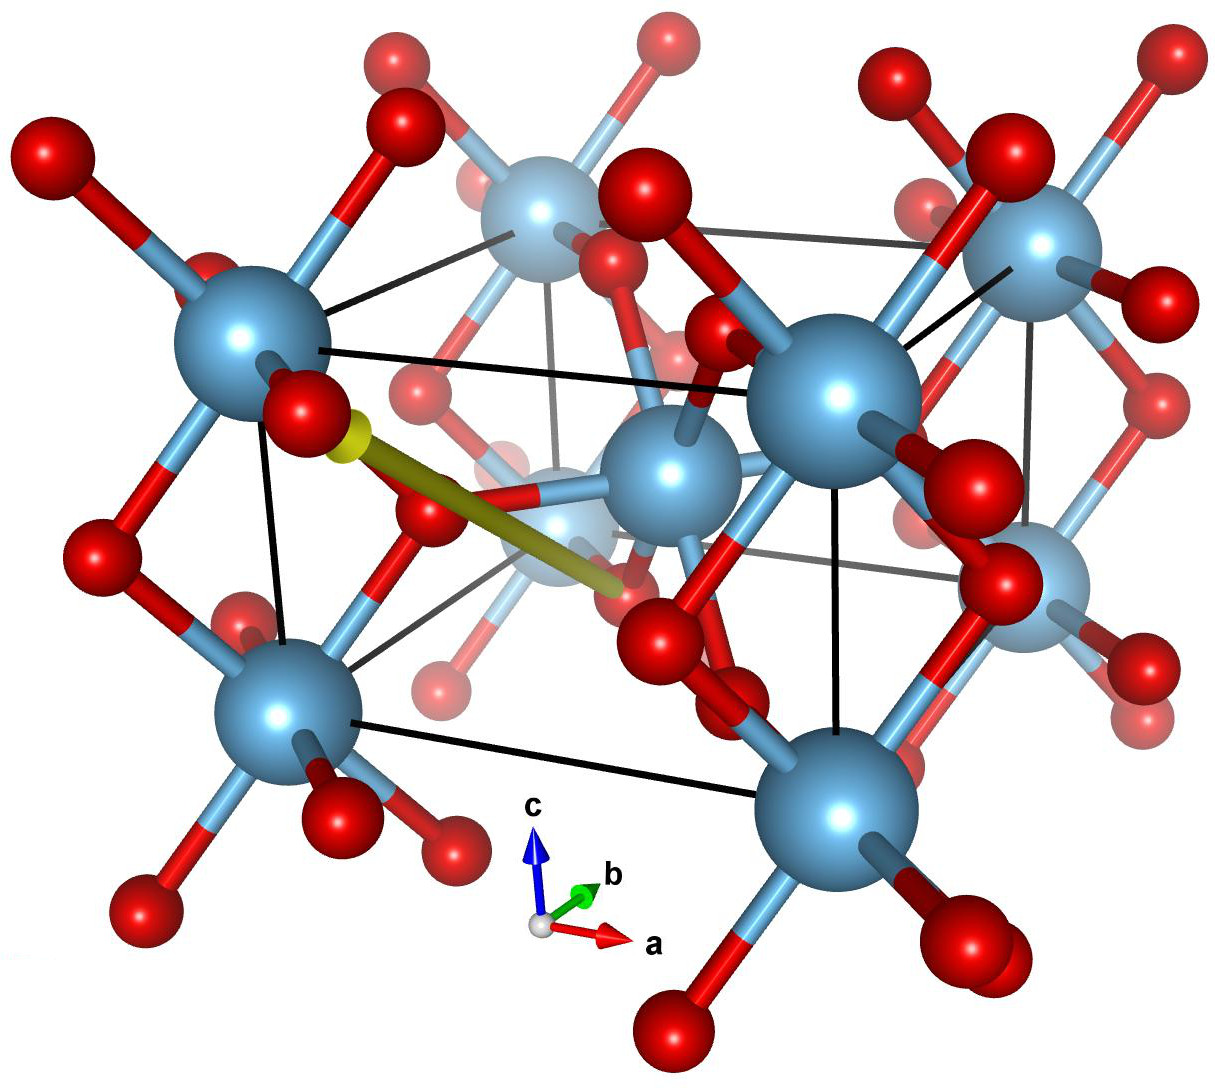
\includegraphics[width=0.45\textwidth]{img/TiO2-rutile-vector.jpg}
   \caption{Unit cell of TiO$_2$-rutile. The $[0\bar{1}1]$ vector, connecting two equivalent oxygen sites, is featured in yellow.}
   \label{fig:rutile-vector} 
  \end{center}
 \end{figure}
\end{center}

The second observation is that in the resulting Magnéli structure, after performing the operations given by equations \ref{eq:transf} and \ref{eq:displ}, some titanium atoms are displaced to interstitial positions with respect to neighboring Ti chains. This can be better visualized in figures \ref{fig:structures-c-prl} (a) and (b), where in the first case, for the TiO$_2$ structure, one can see straight Ti chains along the $c$ vector while in the second case, the Ti$_4$O$_7$ Magnéli structure presents discontinuities in the same chains where interstitial atoms are present. An important detail is that the Ti chains are periodically displaced as if the Ti atoms at their ends were in interstitial positions---and this is exactly where one finds the shear planes---with respect to the neighboring chains along the $c$ direction.
\begin{center}
 \begin{figure}[ht!]
  \begin{center}
   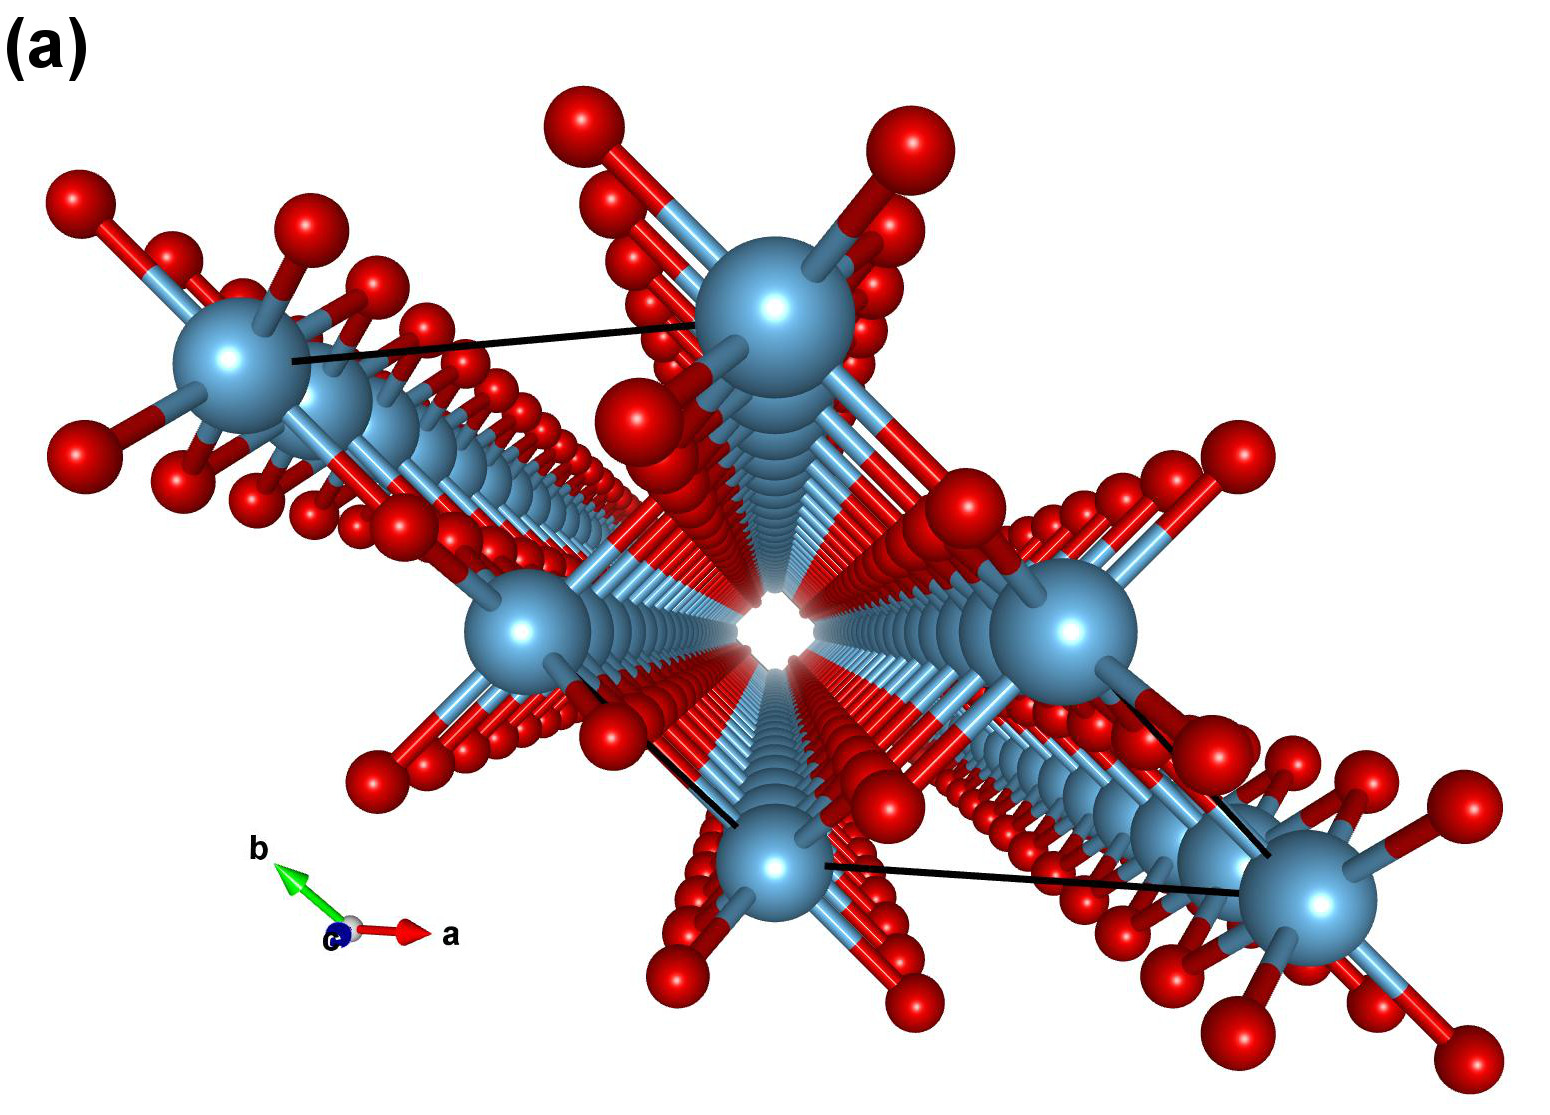
\includegraphics[width=0.45\textwidth]{img/TiO2-c-prl.jpg}
   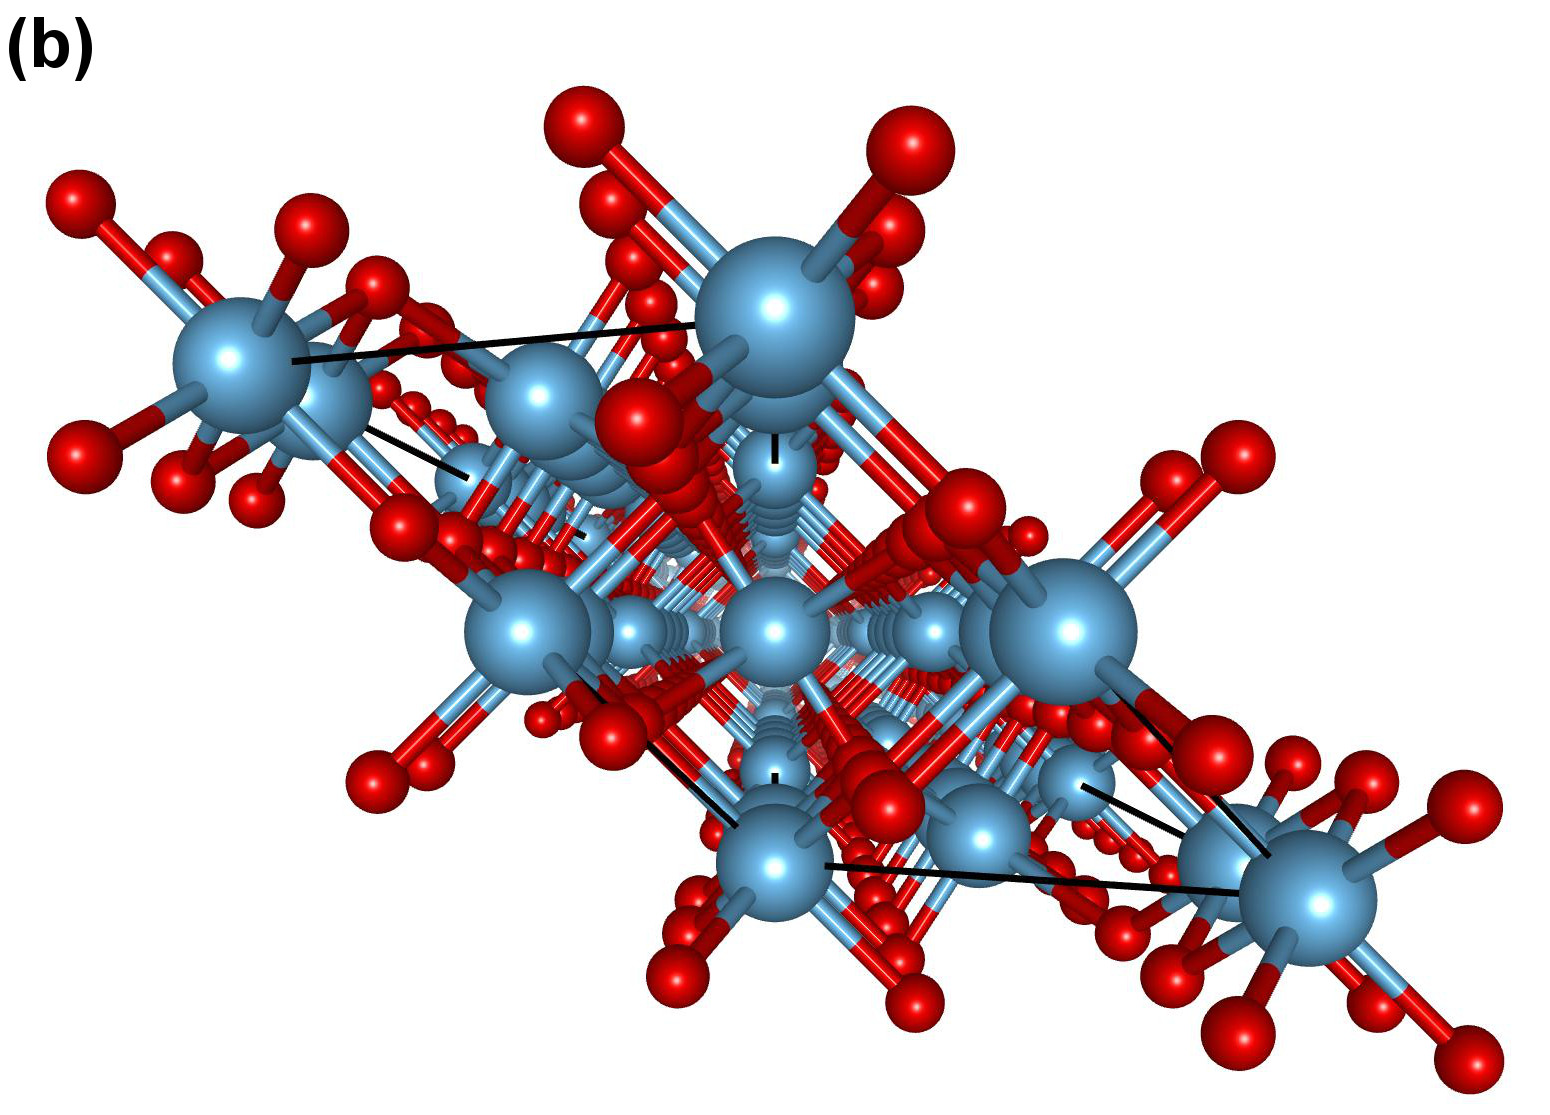
\includegraphics[width=0.45\textwidth]{img/Ti4O7-c-prl.jpg}
   \caption{Structures of (a) TiO$_2$-rutile, and (b) Ti$_4$O$_7$ Magnéli view along the $c$ axis.}
   \label{fig:structures-c-prl} 
  \end{center}
 \end{figure}
\end{center}

These observations are crucial to determine that it is indeed equation \ref{eq:interstitial} which best describes the formation of the Magnéli phases, thus, the whole process can be regarded as the insertion of Ti atoms into the rutile structure.

\section{Formation Enthalpies}
\label{sec:formation}

For the calculation of the formation enthalpies $\Delta H_f^D$ for the Ti$_2$O$_3$-corundum, and Ti$_4$O$_7$ and Ti$_5$O$_9$ Magnéli phases, reservoirs of atoms at constant chemical potential $\mu_{\alpha}$ ($\alpha = \text{Ti}, \text{O}$) and electrons with the potential at $E_F$ were considered, and the unit cell was kept fixed while ionic relaxation was allowed. The expression for $\Delta H_f^D$ with respect to TiO$_2$-rutile, the host material, is given by,
\begin{align}
	\label{eq:e-form-isolated}
	\Delta H_f^D (E_F, \mu, q) &= E_D(q) - E_H + \sum_{\alpha} m_{\alpha} \mu_{\alpha} + \nonumber \\
							   &+ q (E_F + E_{VBM} + \Delta V),
\end{align}
where $E_H$ and $E_D(q)$ stands for the total energy of the system before (TiO$_2$) and after (Ti$_n$O$_{2n-1}$) exchange of $m_{\alpha}$ atoms and $q$ electrons with the respective reservoirs. VBM energy ($E_{VBM}$) is obtained from the bulk TiO$_2$ while $\Delta V$ is an energy shift obtained from core level eigenvalues. 

\begin{center}
 \begin{figure}[ht!]
  \begin{center}
   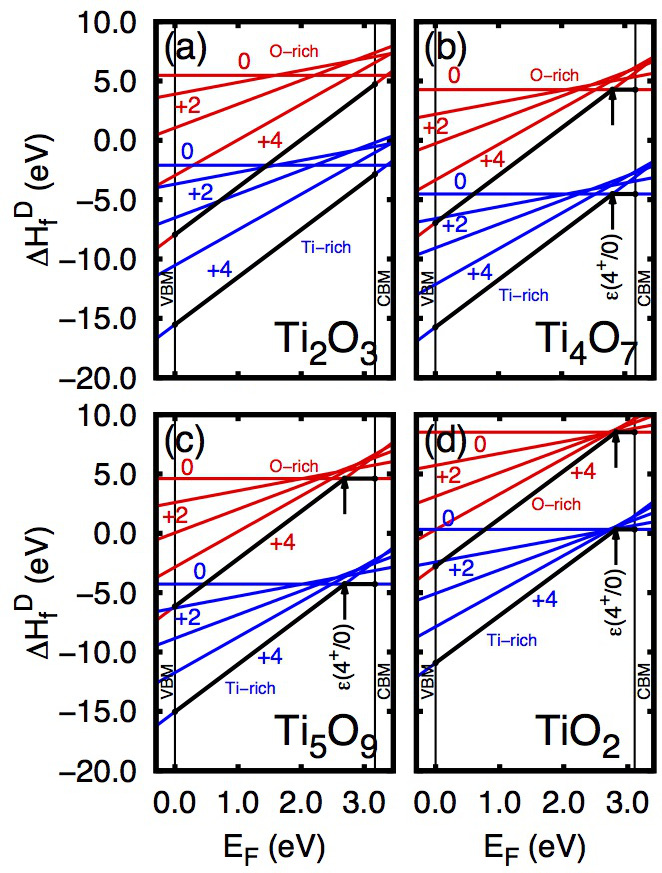
\includegraphics[width=0.75\textwidth]{img/e-form-all.jpg}
   \caption{Formation enthalpies for (a) Ti$_2$O$_3$, (b) Ti$_4$O$_7$, (c) Ti$_5$O$_9$, and (d) Ti$_i$ point defect in TiO$_2$-rutile. Each line is the plot of the formation enthalpy for a different charge state, which is the slope, according to equation \ref{eq:e-form-isolated}. The thick black lines feature the lowest energy for each occupation across the bandgap ($E_F$) while the charge transitions are featured by the black arrows.}
   \label{fig:e-form-full} 
  \end{center}
 \end{figure}
\end{center}

According to the discussion in the previous section, in this case one should consider the case where only Ti atoms are inserted into the structure, thus, $\alpha = \text{Ti}$ and $m_{\alpha} = +1$ for the unit cell used in our calculations. This quantity is plotted for each charge state from neutral up to $+4$, given that Ti atoms present oxidation numbers ranging in this interval. The results for the three oxygen-deficient phases are compared with the same quantity obtained for the Ti$_i$ point defect from the literature \cite{Lee2012}, and are presented in figure \ref{fig:e-form-full}. O-rich and Ti-rich conditions are the limiting cases for the $\mu_{\text{Ti}}$, which are given by the stability condition.

From these graphs it is noticeable that Ti$_2$O$_3$ presents a fully ionized state ($q = +4$) as the most stable one across the whole span of the bandgap. This means that, when in the vicinity of TiO$_2$-rutile, this compound is stabilized by donating its four electrons per unit cell. While the same situation happens for most of the bandgap, in the case of Ti$_4$O$_7$ and Ti$_5$O$_9$ there is a transition from $+4$ to neutral state close to $E_{CBM}$: $\varepsilon(+4/0) = E_{CBM} - 0.36$ eV and 0.48 eV respectively. This is very similar to what happens in the case of Ti$_i$, where the same charge transition lies close to the same region: $\varepsilon(+4/0) = E_{CBM} - 0.29$ eV. Thus, these oxygen-deficient structures, which present no crystallographic defects---these are new crystals---behave similarly to Ti$_i$ point defects from an electronic structure point of view. For this reason, we choose to refer to these systems as containing \textit{pseudodefects}. Moreover, the abrupt transition from  $+4$ to neutral state and the large structural relaxation present is a strong evidence of a negative-$U$ behavior \cite{Watkins1984}.

\section{Charge storage}
\label{sec:charge-storage}

The charged states in the Ti$_4$O$_7$ and Ti$_5$O$_9$ structures were investigated by means of the PDOS, presented in figure \ref{fig:pdos-charged}. For each charge state a graph was plotted aiming to understand the changes in the electronic levels due to charging. It is possible to see that the electrons are removed from an \textit{intermediate band} inside the bandgap. As electrons are removed, the most energetic occupied level increases in energy. This effect is more pronounced in the Ti$_4$O$_7$ PDOS but still present in the Ti$_5$O$_9$ case. The consequence of that increase is that the system will switch from the neutral state directly to $+4$ state as long as the Fermi energy is enough lowered by an external perturbation, for example an electrode subject to a given potential.
\begin{center}
 \begin{figure}[ht!]
  \begin{center}
   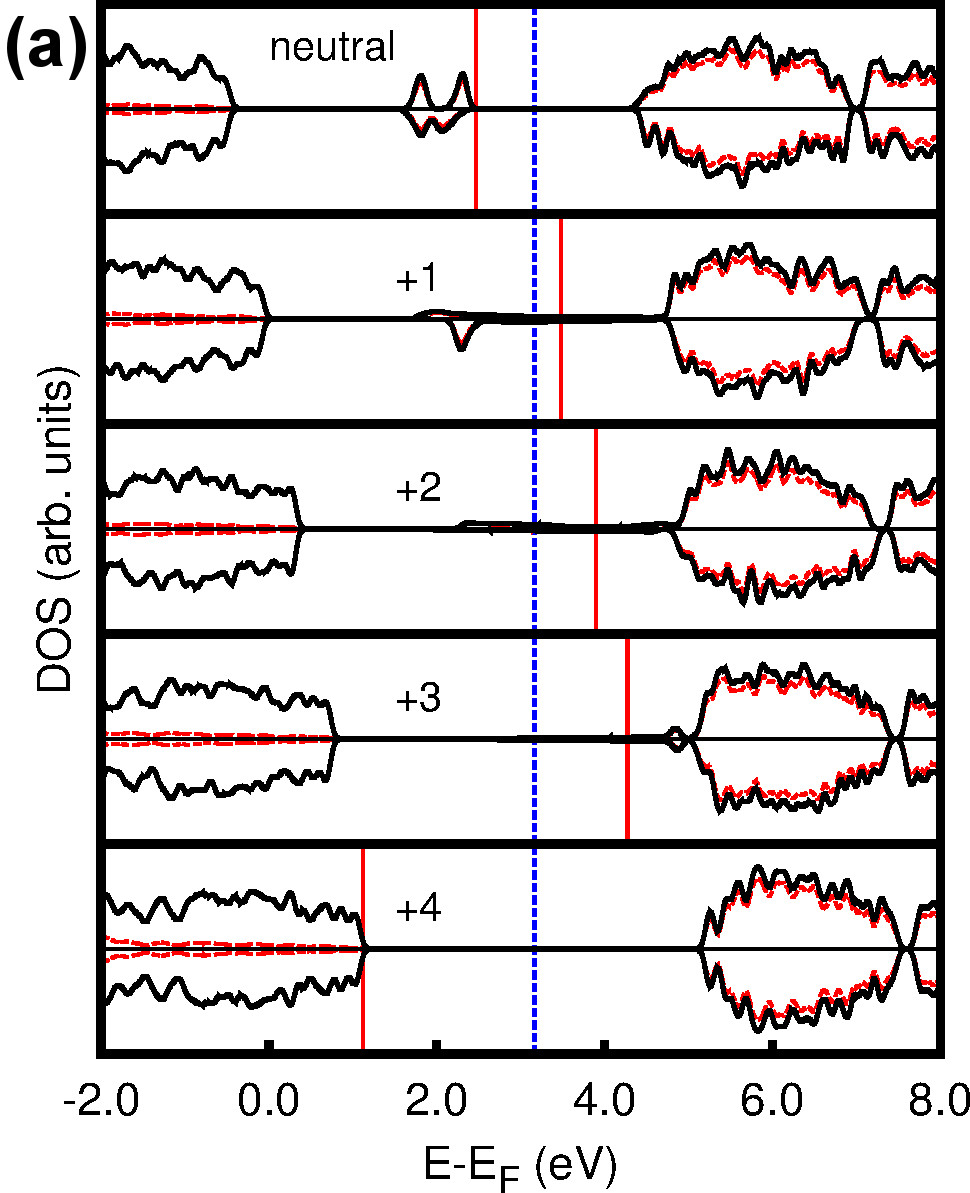
\includegraphics[width=0.45\textwidth]{img/dos-ti4o7-prl-ef.jpg}
   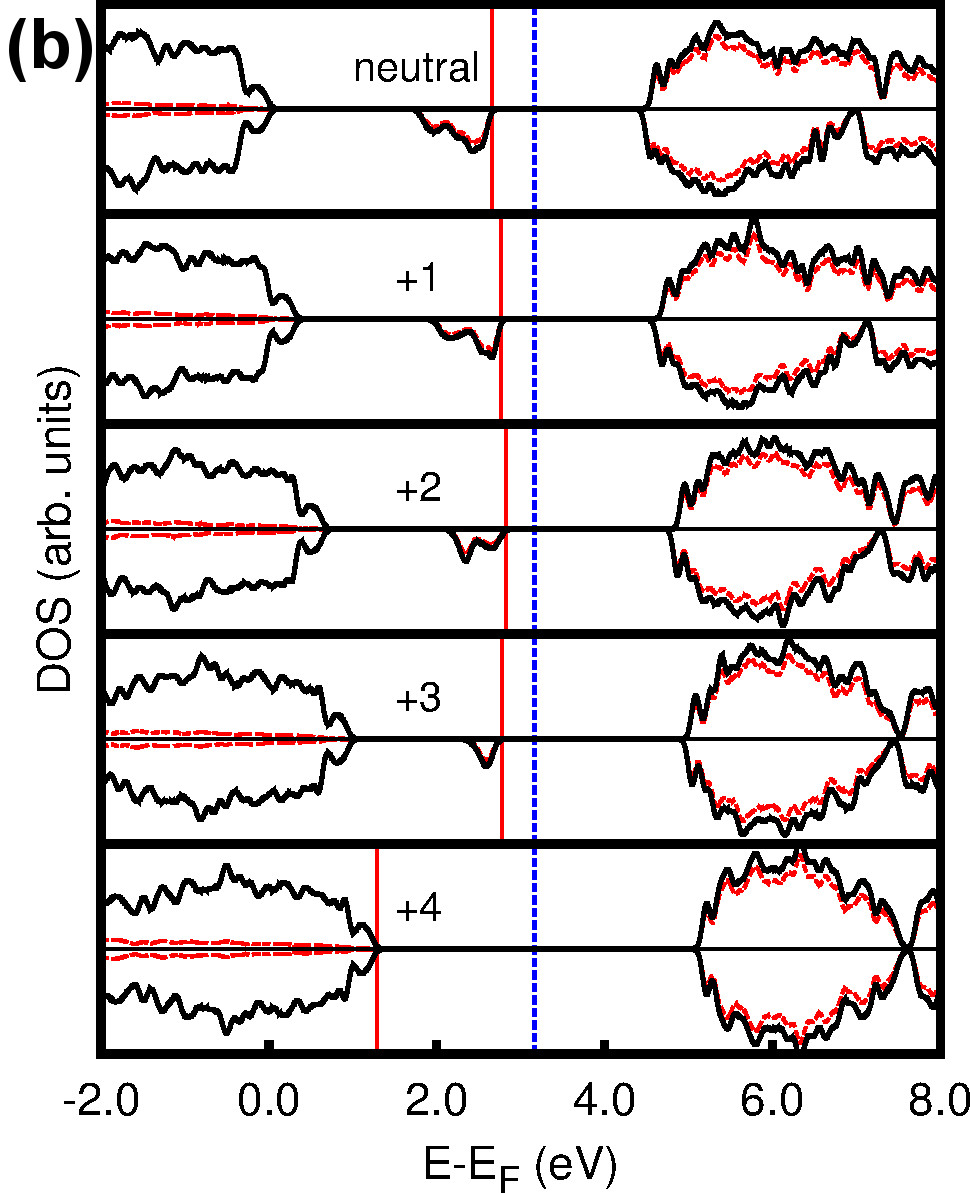
\includegraphics[width=0.45\textwidth]{img/dos-ti5o9-prl-ef.jpg}
   \caption{PDOS for all charge states of (a) Ti$_4$O$_7$, and (b) Ti$_5$O$_9$. The full black line is the total DOS while the red dashed line is the Ti(d) contribution. The positive and negative values along the vertical axis are the spin components, the vertical red line is the last occupied level and the dashed blue vertical line is the TiO$_2$ CBM. Energies are referenced from the TiO$_2$ VBM.}
   \label{fig:pdos-charged} 
  \end{center}
 \end{figure}
\end{center}

In fact, 3d transition metal-related defects in semiconductors exhibit multiple charge states \cite{Haldane1976}, even in the case where these defects are extended \cite{Raebiger2014}. Cation defects in MnO$_2$ where reported to introduce switching states, which could be used to store charge \cite{Young2015}. In the case of the Magnéli phases presented here, the same switching states are present, but due to an intermediate band introduced by pseudodefects, instead of localized states introduced by point defects. The real-space projection of the intermediate band is presented in figure \ref{fig:ti5o9-parchg-prl}, where it is possible to see that the band is delocalized over several Ti atoms of the structure.
\begin{center}
 \begin{figure}[ht!]
  \begin{center}
   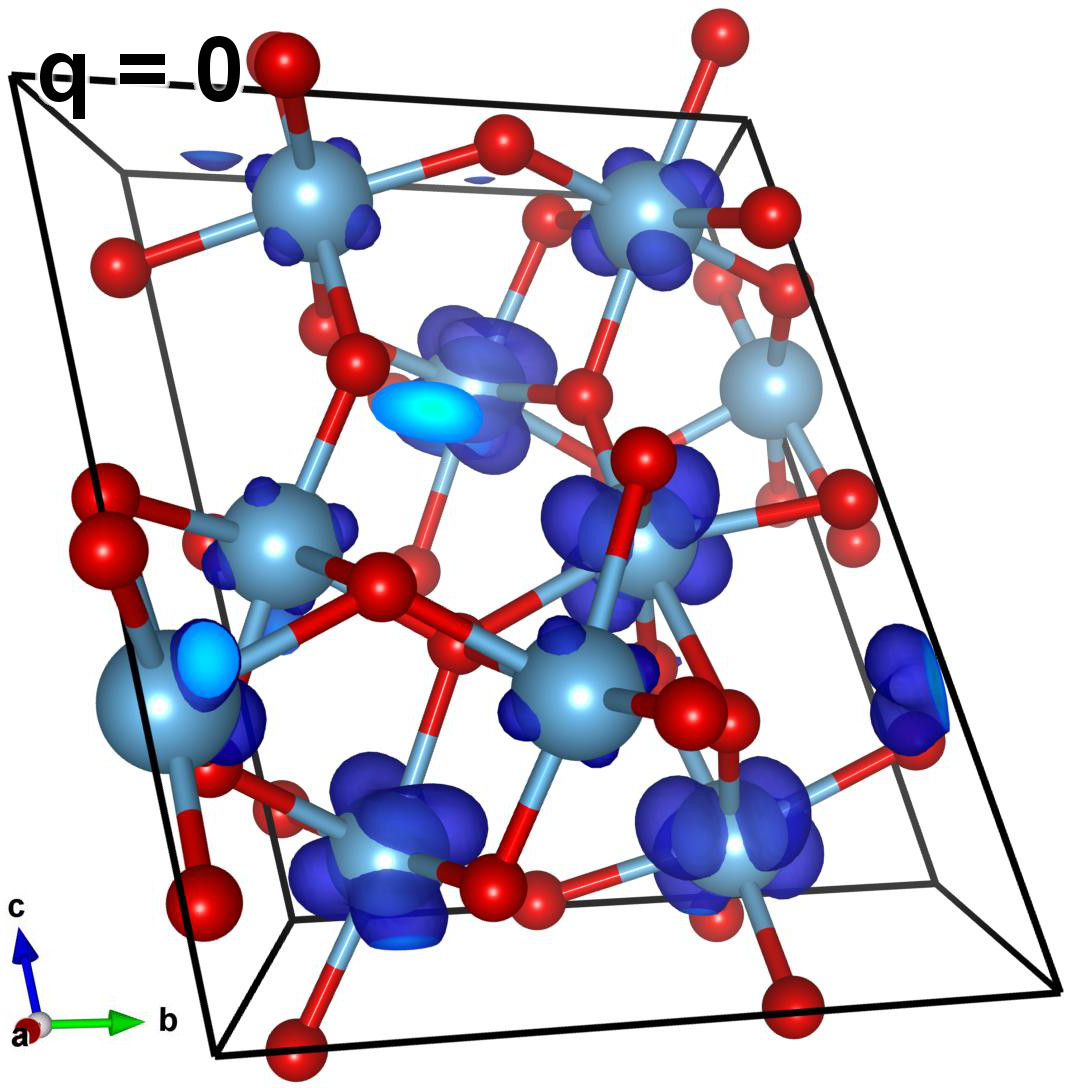
\includegraphics[width=0.18\textwidth]{img/ti5o9-q0-parchg-prl.jpg}
   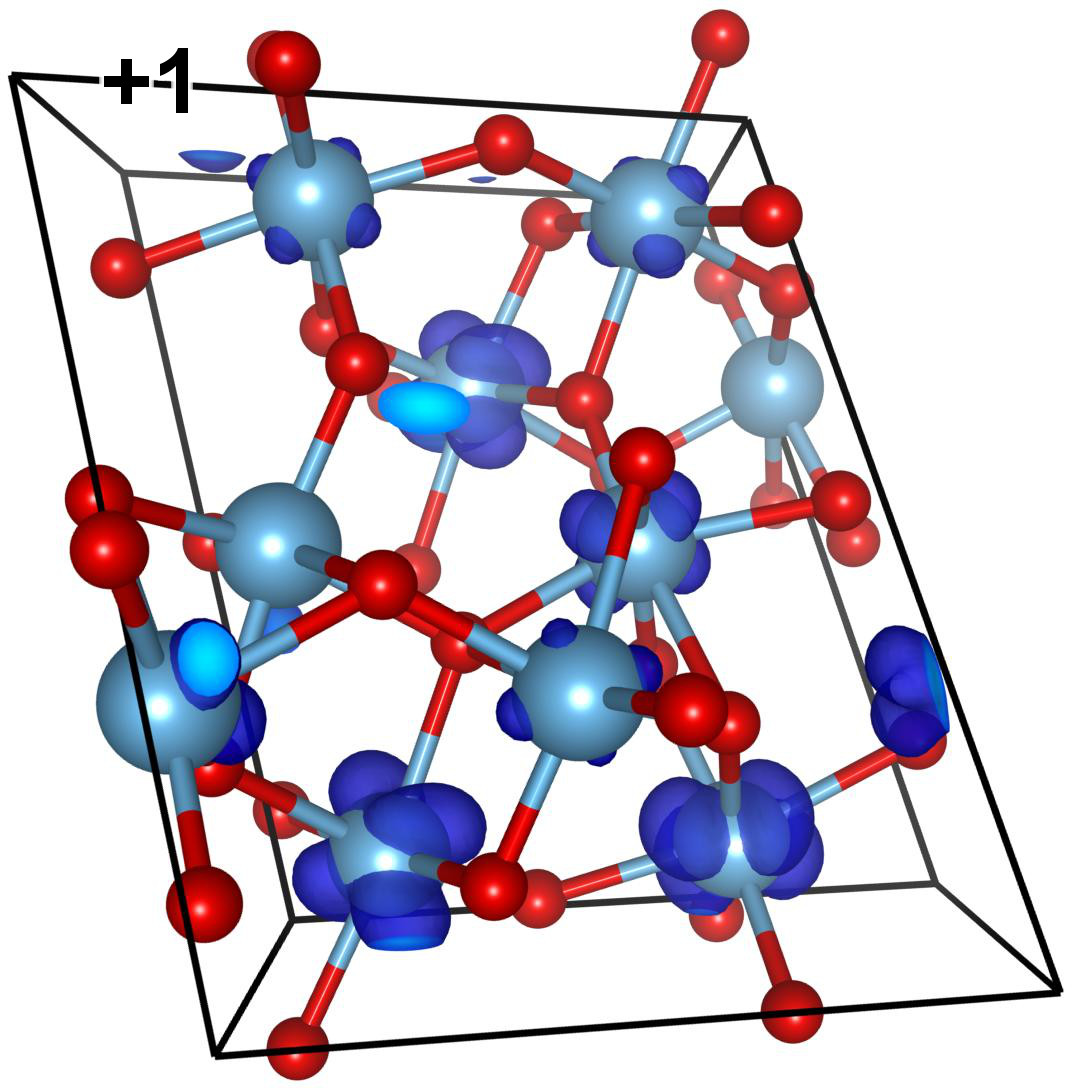
\includegraphics[width=0.18\textwidth]{img/ti5o9-q1-parchg-prl.jpg}
   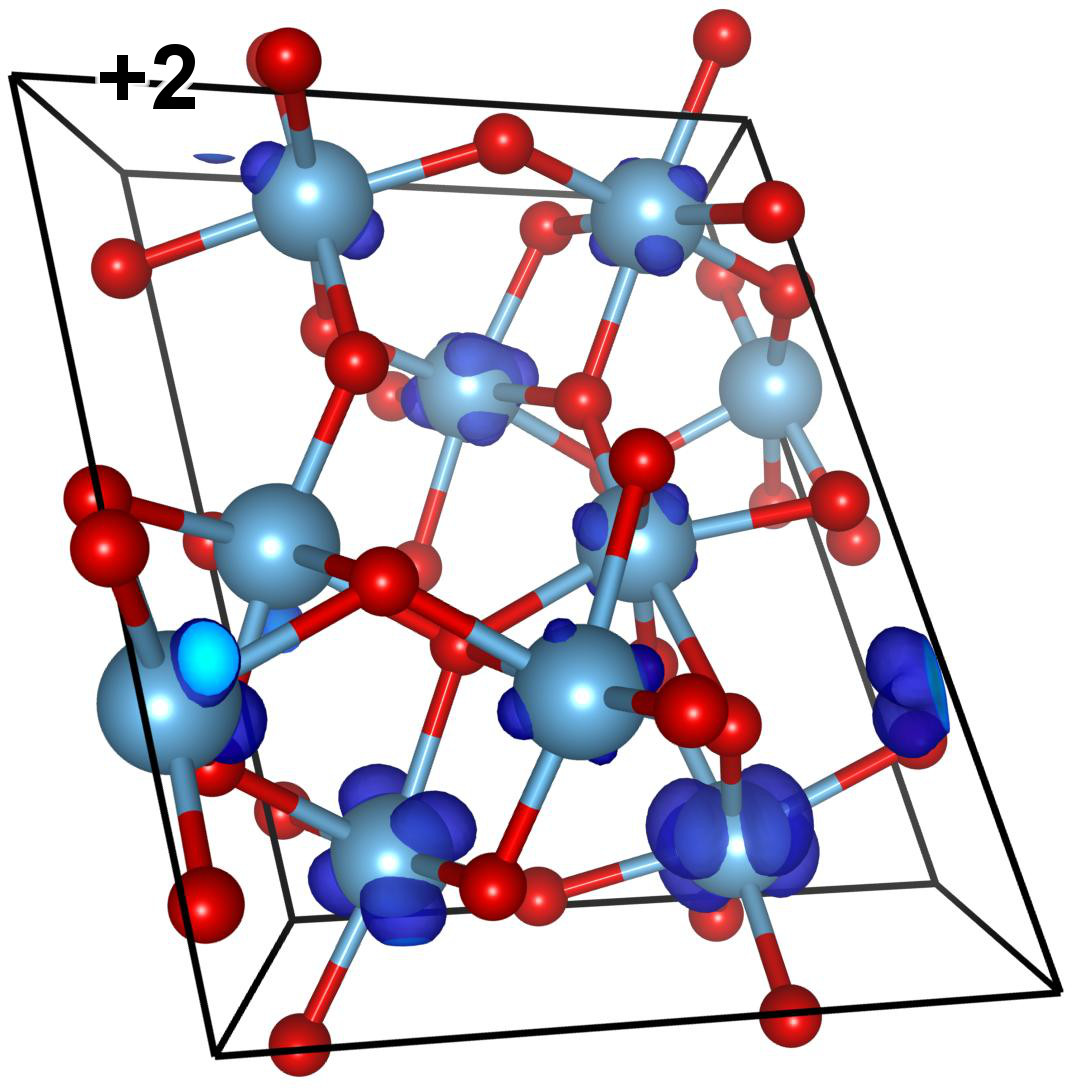
\includegraphics[width=0.18\textwidth]{img/ti5o9-q2-parchg-prl.jpg}
   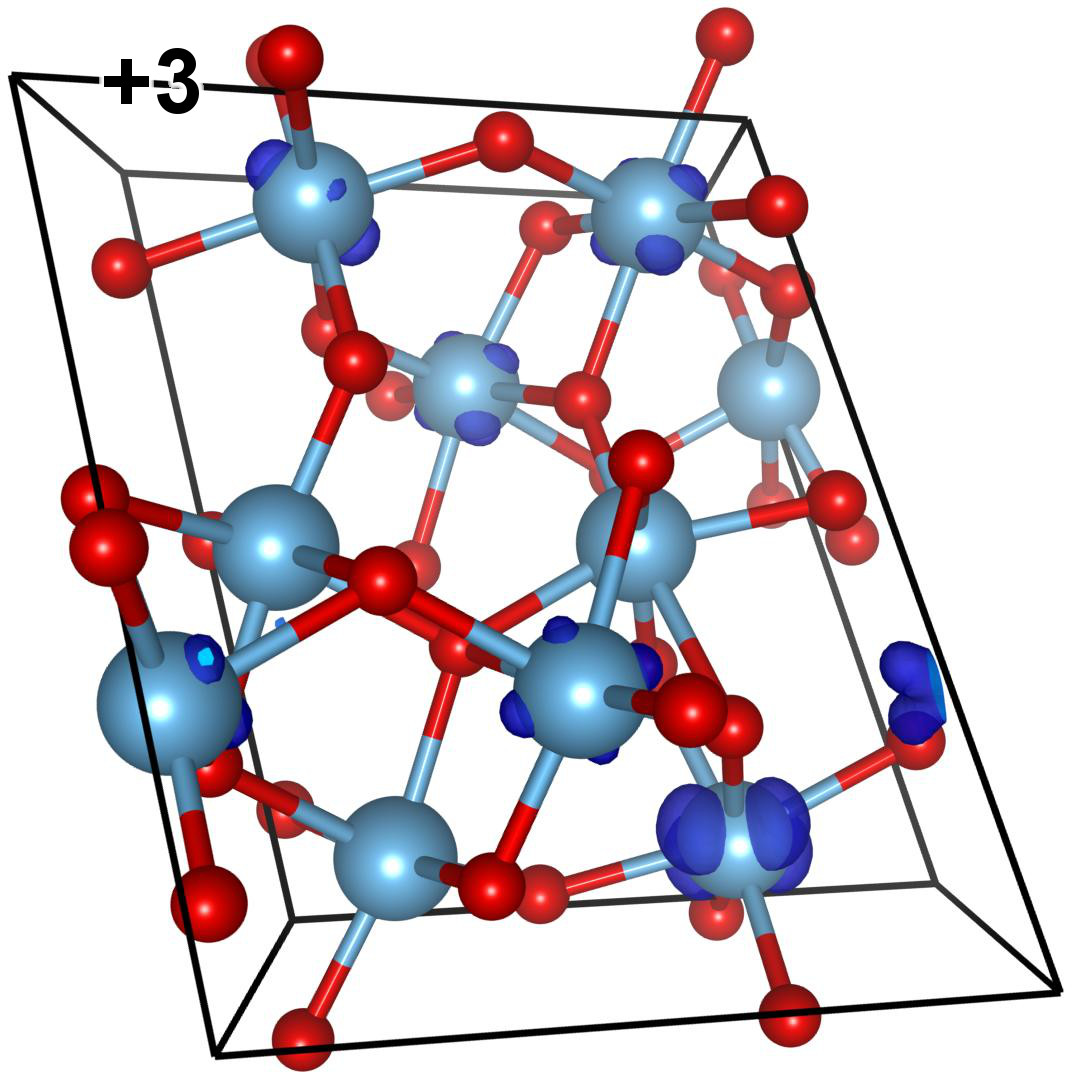
\includegraphics[width=0.18\textwidth]{img/ti5o9-q3-parchg-prl.jpg}
   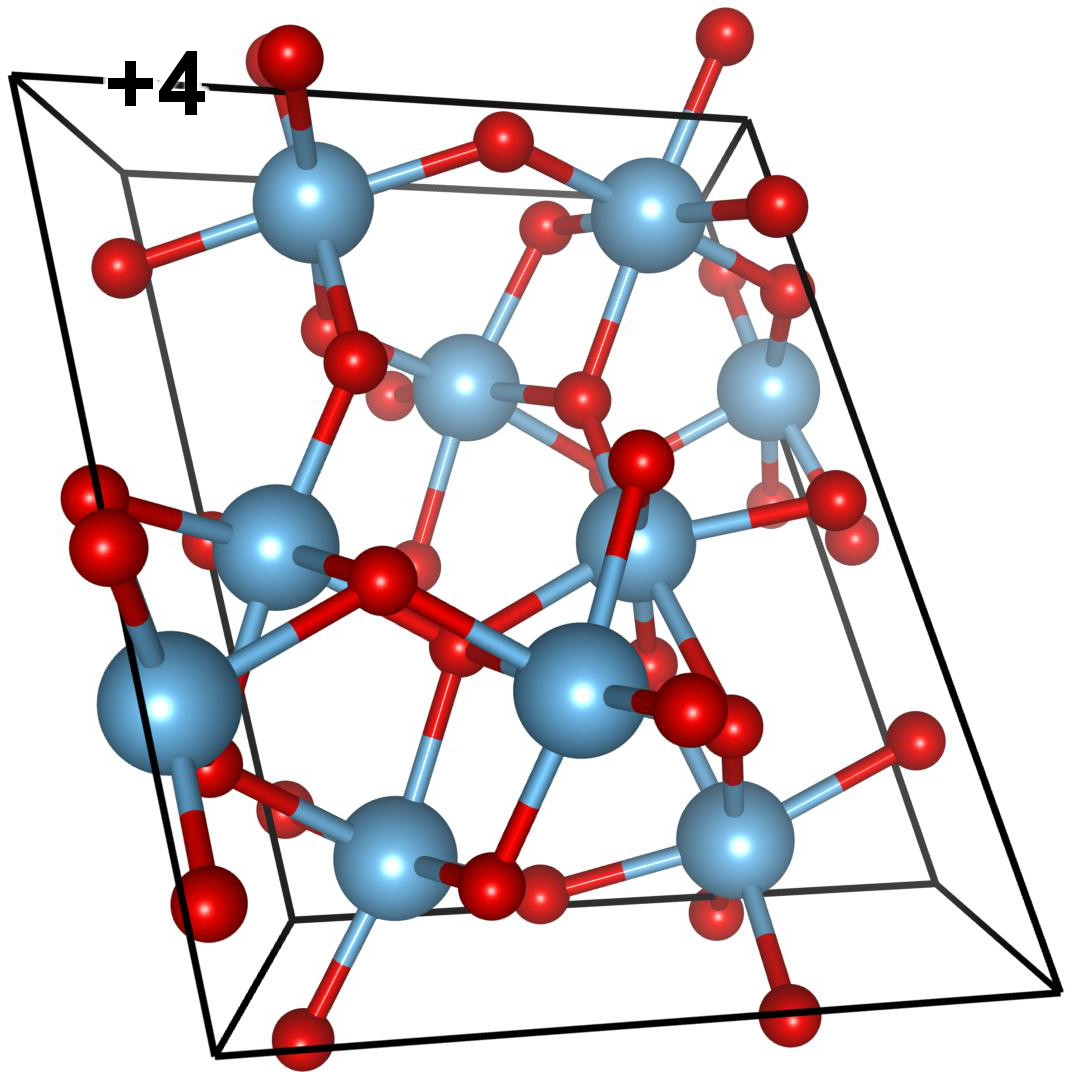
\includegraphics[width=0.18\textwidth]{img/ti5o9-q4-parchg-prl.jpg}
   \caption{Real-space projection of the intermediate band of Ti$_5$O$_9$ for all studied charge states. The isosurface chosen was $10^{-2}e\cdot \text{Bohr}^{-3}$ while the energy range was $E_F - 1.5 \, \text{eV} < E < E_F$. For the $+4$ state the structure is presented only for completion, once it presents no intermediate band.}
   \label{fig:ti5o9-parchg-prl} 
  \end{center}
 \end{figure}
\end{center}

In conclusion, these systems could be charged and de-charged if a proper setup of electrodes is provided, just as it is the case of the memristors. The switching is then closely related to this charge storage mechanism, and additionally, a charge storage application is possible. Given the fact that the Magnéli phases studied here can donate 4 electrons per unit cell, we estimate that the maximum charge storage capability of a device made of these materials operating at 1 V is 600 F/g for Ti$_4$O$_7$ and 500 F/g for Ti$_5$O$_9$, which places these devices as possible supercapacitors. These results have been submitted for publication and the manuscript is attached in appendix \ref{sec:app-sub}.
